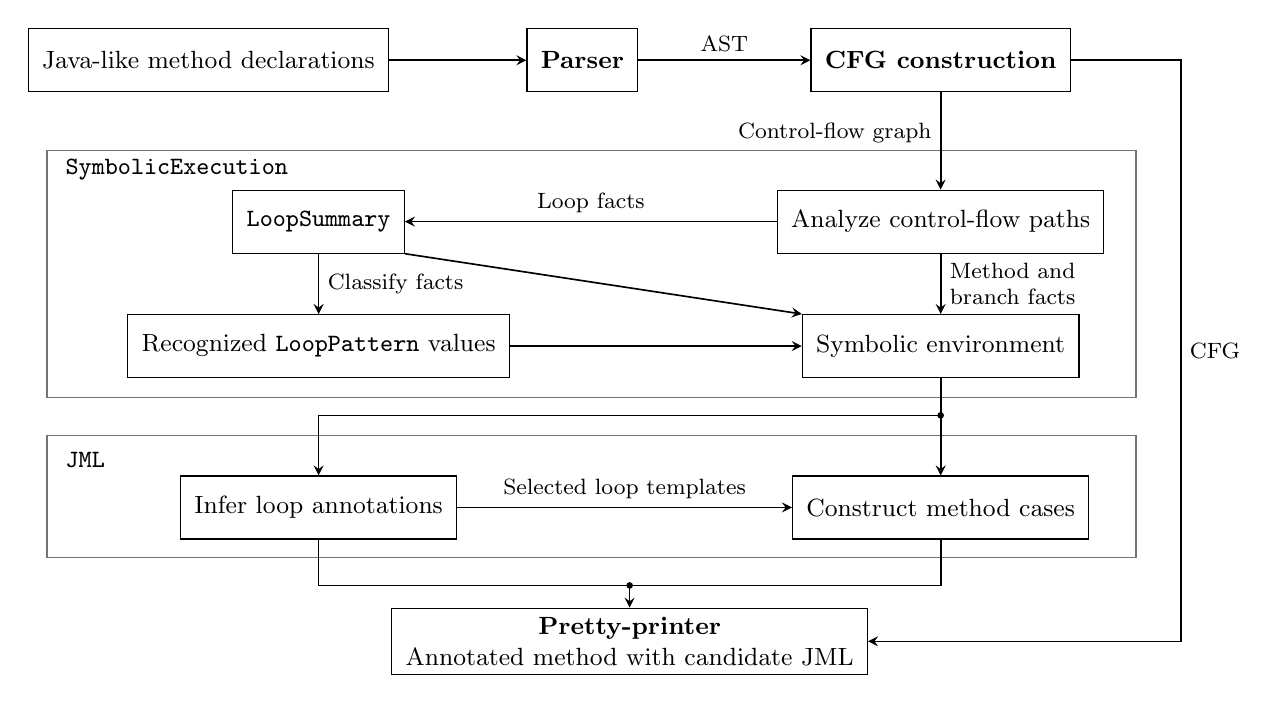
\begin{tikzpicture}[
  font=\small,
  stage/.style={draw, align=center, minimum height=8mm, inner xsep=5pt},
  module/.style={draw=black!55, thin},
  module title/.style={anchor=west, inner sep=0pt, font=\small\bfseries},
  flow/.style={->, >=stealth, semithick},
  edge label/.style={font=\footnotesize, align=center, inner sep=3pt}
]
  \node[stage] (source) at (-5.35,0) {Java-like method declarations};
  \node[stage] (parser) at (-0.6,0) {\textbf{Parser}};
  \node[stage] (cfg) at (3.95,0) {\textbf{CFG construction}};
  \draw[flow] (source) -- (parser);
  \draw[flow] (parser) -- node[edge label, above] {AST} (cfg);

  \draw[module] (-7.4,-1.15) rectangle (6.43,-4.28);
  \node[module title] at (-7.17,-1.39) {\texttt{SymbolicExecution}};
  \node[stage] (traverse) at (3.95,-2.05) {Analyze control-flow paths};
  \node[stage] (summary) at (-3.95,-2.05) {\texttt{LoopSummary}};
  \node[stage] (patterns) at (-3.95,-3.63) {Recognized \texttt{LoopPattern} values};
  \node[stage] (environment) at (3.95,-3.63) {Symbolic environment};
  \draw[flow] (cfg) -- node[edge label, pos=.42, left] {Control-flow graph} (traverse);
  \draw[flow] (traverse) -- node[edge label, above] {Loop facts} (summary);
  \draw[flow] (summary) -- node[edge label, right] {Classify facts} (patterns);
  \draw[flow] (traverse) -- node[edge label, right] {Method and\\branch facts} (environment);
  \draw[flow] (summary.south east) -- (environment.north west);
  \draw[flow] (patterns) -- (environment);

  \draw[module] (-7.4,-4.77) rectangle (6.43,-6.31);
  \node[module title] at (-7.17,-5.07) {\texttt{JML}};
  \node[stage] (loop) at (-3.95,-5.68) {Infer loop annotations};
  \node[stage] (method) at (3.95,-5.68) {Construct method cases};
  \coordinate (inference) at (3.95,-4.51);
  \draw[flow] (environment) -- (method);
  \draw[flow] (inference) -| (loop);
  \fill (inference) circle[radius=1.2pt];
  \draw[flow] (loop) -- node[edge label, above] {Selected loop templates} (method);

  \node[stage] (render) at (0,-7.38) {\textbf{Pretty-printer}\\Annotated method with candidate JML};
  \coordinate (annotations) at (0,-6.67);
  \draw[semithick] (loop.south) |- (annotations) -| (method.south);
  \draw[flow] (annotations) -- (render.north);
  \fill (annotations) circle[radius=1.2pt];
  \draw[flow] (cfg.east) -- (7.0,0) |-
    node[edge label, pos=.25, right] {CFG} (render.east);
\end{tikzpicture}
